\section{Principio de Funcionamiento}
\label{principio}

El fen\'omeno f\'isico en que se basa el m\'aser es la emisi\'on estimulada de radiaci\'on. Antes de explicar este fen\'omeno repasaremos algunas propiedades de la materia y algunos t\'erminos relacionados con la mec\'anica cu\'antica que facilitar\'an posteriormente su comprensi\'on.

\subsection{Conceptos b\'asicos}

Algunas propiedades de la materia y la radiaci\'on que intervienen en el funcionamiento del m\'aser son las siguientes \cite{maserEspacio}:

\begin{itemize}
 \item Los \'atomos y las mol\'eculas pueden estar en distintos niveles de energ\'ia.
 \item Un \'atomo o una mol\'ecula que absorba energ\'ia puede pasar a un nivel superior, y an\'alogamente, puede pasar a un nivel inferior liberando la energ\'ia sobrante.
 \item Una forma de caer a un estado inferior es emitir radiaci\'on. La diferencia de energ\'ia entre los niveles determina la longitud de onda emitida. 
 \item En situaciones de equilibrio, la cantidad de part\'iculas de cada nivel est\'a determinada por la temperatura del material. En los materiales m\'as calientes hay m\'as part\'iculas en estados de alta energ\'ia. En cualquier caso, siempre hay m\'as part\'iculas en los estados m\'as bajos.
\end{itemize}

Algunos fen\'omenos que afectan a la interacci\'on entre la materia y la radiaci\'on son la absorci\'on, la emisi\'on espont\'anea y la emisi\'on estimulada:

\begin{itemize}
 \item \textbf{Absorci\'on}

Seg\'un la mec\'anica cu\'antica la absorci\'on de fotones por los \'atomos s\'olo se produce si la longitud de onda del fot\'on es la adecuada (longitud l). Si lo es, el \'atomo lo \textit{absorber\'a} (es decir, el fot\'on se desvanece), y subir\'a un estado de energ\'ia  m\'as alto.

 \item \textbf{Emisi\'on espont\'anea}

Seg\'un las leyes de la termodin\'amica, a los \'atomos \textit{no les gusta} permanecer en niveles altos de energ\'ia, por lo que despu\'es de absorber un fot\'on y subir a un nivel de energ\'ia superior, bajar\'a por s\'i mismo a un nivel inferior emitiendo un fot\'on en el proceso. Este proceso se conoce como emisi\'on espont\'anea porque ninguna influencia externa produce la emisi\'on. Normalmente el tiempo medio para que un \'atomo excitado produzca emisi\'on espont\'anea es unos $10^{-8}$ segundos, es decir, el \'atomo o mol\'ecula tardar\'a unos $10^{-8}$ segundos en emitir el fot\'on. A veces, sin embargo, hay estados en los cuales el \'atomo puede permanecer m\'as tiempo, alrededor de unos $10^{-3}$ segundos. Son los estados conocidos como \textit{metaestables}. Los niveles de emisi\'on metaestable son imprescindibles para el funcionamiento del m\'aser.

Ahora que se han descrito los fen\'omenos de absorci\'on y emisi\'on espont\'anea, vamos a hablar de la emisi\'on estimulada, que es el fen\'omeno que genera el haz m\'aser.

 \item \textbf{Emisi\'on estimulada}

Para que se produzca la emisi\'on estimulada se hace impactar un fot\'on de la longitud de onda de absorci\'on l contra un \'atomo que ya se encontraba en un nivel alto de energ\'ia por una absorci\'on previa. El \'atomo absorber\'a el nuevo fot\'on e inmediatamente emitir\'a dos fotones para volver a su nivel de energ\'ia inicial. Seg\'un dicta la mec\'anica cu\'antica, estos dos fotones emitidos tendr\'an la misma longitud de onda, l. 

\begin{figure}[htb!!]
 \centering
 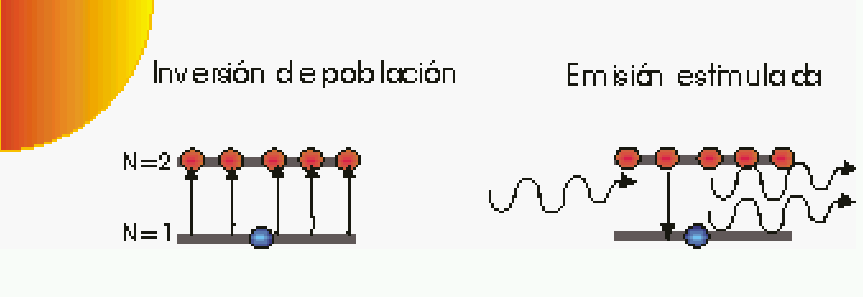
\includegraphics[width=0.7\textwidth,keepaspectratio=true]{./Utils/emision_estimulada.png}
 % emision_estimulada.png: 863x297 pixel, 101dpi, 21.71x7.47 cm, bb=0 0 615 212
 \caption{Inversión de población y emisión estimulada}
 \label{fig:emision_estimulada}
\end{figure}

En la Figura \ref{fig:emision_estimulada} se muestra el proceso de inversi\'on de la poblaci\'on y emisi\'on estimulada. La inversi\'on de la poblaci\'on consiste en excitar los \'atomos de forma que haya m\'as en el nivel de energ\'ia alto que en el bajo, y despu\'es se hace incidir un fot\'on, lo que provoca la emisi\'on de dos fotones con la misma longitud de onda.

\end{itemize}

\subsection{Funcionamiento del m\'aser}

En la Figura \ref{fig:funcionamiento_maser} se describe el funcionamiento del m\'aser. En la imagen las mol\'eculas excitadas, es decir, en un nivel alto de energ\'ia, se representan con c\'irculos rojos, y los peque\~nos c\'irculos azules representan mol\'eculas en un nivel bajo de energ\'ia.

En las im\'agenes A y B vemos c\'omo un grupo de mol\'eculas es excitado por radiaci\'on o choques, de forma que pasan a un nivel alto de energ\'ia. En C un fot\'on incide por la izquierda a estas mol\'eculas. En D, el fot\'on estimula la emisi\'on de la primera mol\'ecula, que libera la energ\'ia retenida en el paso A. Como resultado se obtienen dos fotones de longitud de onda l (en fase) y una mol\'ecula en un nivel bajo de energ\'ia. Estos dos fotones liberados estimulan la emisi\'on de las dos mol\'eculas siguientes (E), en un proceso que contin\'ua en forma de reacci\'on en cadena, doblando el n\'umero de fotones muy r\'apidamente (F).

\begin{figure}[htb!!]
 \centering
 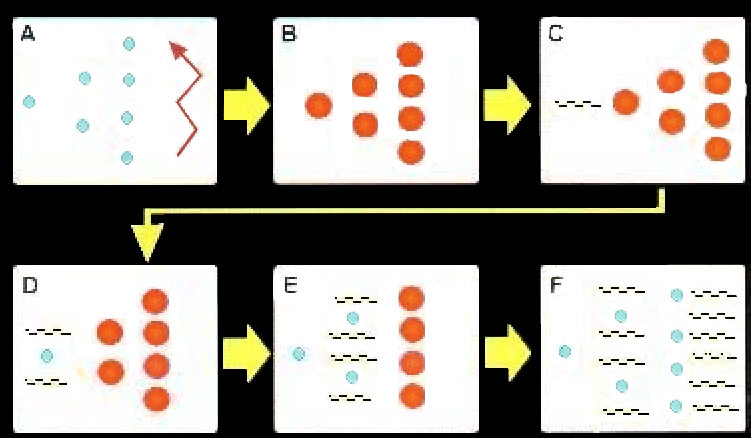
\includegraphics[width=0.9\textwidth]{./Utils/maser_funcionamiento2.png}
 % emision_estimulada.png: 863x297 pixel, 101dpi, 21.71x7.47 cm, bb=0 0 615 212
 \caption{Inversión de población y emisión estimulada}
 \label{fig:funcionamiento_maser}
\end{figure}

Como se ha indicado anteriormente, para que un material produzca emisi\'on m\'aser debe romperse su equilibrio natural. Inyectando energ\'ia en el material se puede conseguir una inversi\'on de la poblaci\'on entre dos niveles, es decir, que haya m\'as \'atomos o mel\'eculas en el nivel de energ\'ia superior. Mientras dura esta inversi\'on, se hace pasar radiaci\'on con la longitud de onda que corresponda a la diferencia de energ\'ia entre dos niveles, y de este modo se estimula una ca\'ida s\'ubita de las part\'iculas del nivel superior al inferior, produciendo un potente fogonazo de microondas. De esta forma se consigue un haz de radiaci\'on intenso, estrecho y monocrom\'atico (es decir, con una \'unica longitud de onda). 

Adem\'as de los m\'aseres artificiales (creados por el hombre), tambi\'en se producen m\'aseres de forma natural en el universo. Son los m\'aseres astron\'omicos, en los que una estrella act\'ua como fuente de energ\'ia, consiguiendo la inversi\'on de la poblaci\'on en un grupo de mol\'eculas. Estos grupos de mol\'eculas son habitualmente nubes moleculares en las que se est\'an formando estrellas o envolturas estelares. Este fen\'omeno nos permite detectar estrellas que de otro modo ser\'ian indetectables porque su emisi\'on espont\'anea es demasiado d\'ebil.
